\documentclass{standalone}
\usepackage{tikz}

\begin{document}
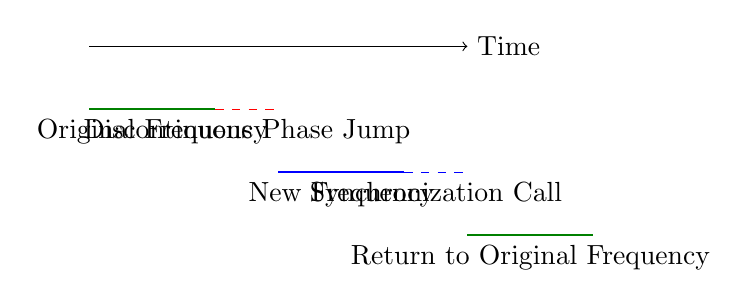
\begin{tikzpicture}[scale=0.8]
    % Define colors for clarity
    \definecolor{original}{RGB}{0,128,0} % Green for original frequency
    \definecolor{new}{RGB}{0,0,255}     % Blue for new frequency

    % Time axis
    \draw[->] (0,0) -- (6,0) node[right] {Time};

    % Original frequency waveform
    \draw[thick, original] (0,-1) -- (2,-1);
    \node at (1,-1) [below] {Original Frequency};

    % Discontinuous phase jump
    \draw[dashed, red] (2,-1) -- (3,-1);
    \node at (2.5,-1) [below] {Discontinuous Phase Jump};

    % New frequency waveform
    \draw[thick, new] (3,-2) -- (5,-2);
    \node at (4,-2) [below] {New Frequency};

    % Synchronization call
    \draw[dashed, blue] (5,-2) -- (6,-2);
    \node at (5.5,-2) [below] {Synchronization Call};

    % Return to original frequency
    \draw[thick, original] (6,-3) -- (8,-3);
    \node at (7,-3) [below] {Return to Original Frequency};
\end{tikzpicture}
\end{document}